\subsection{Sensors}

\subsubsection{Landmine Detection Techniques}

Landmine detection technologies have evolved to encompass a wide range of sensing principles, each targeting specific physical, chemical, or biological characteristics of surface-laid and buried mines. Broadly, these methods can be categorized into five general classes: \textit{\textbf{electromagnetic induction-based} techniques}, \textit{\textbf{radiowave and microwave-based} systems}, \textit{\textbf{mechanical and vibro-acoustic} methods}, \textit{\textbf{spectral and thermal imaging} approaches}, and \textit{\textbf{chemical and biological} sensing methods}. Within each class, a variety of specialized detection technologies have been developed, including traditional metal detectors, ground-penetrating radar, infrared and hyperspectral imaging, seismic/acoustic sensors, vapor detection, and biosensors. Each of these approaches offers distinct advantages and faces specific limitations, especially when adapted to drone-based platforms for remote and efficient minefield scanning. In the following subsections, each class is explored in detail, with emphasis on the operating principles, detection capabilities, challenges, and documented UAV-based applications.

\paragraph{Electromagnetic Induction-Based Techniques}

Electromagnetic induction (EMI) methods operate by exploiting the interaction between electromagnetic fields and conductive or magnetic materials in the ground. These systems are typically composed of a transmitter coil that emits a time-varying electromagnetic field into the soil. When this field encounters a conductive object—such as a landmine with metallic components—it induces eddy currents within the object, which in turn generate a secondary magnetic field. This field is detected by a receiver coil, and the resulting signal is processed to infer the presence of the object. These principles form the basis of conventional \textbf{metal detectors}~\cite{gichd2006guidebook}.

In contrast, \textbf{magnetic sensors} or magnetometers do not actively induce eddy currents but instead measure disturbances in the Earth's ambient magnetic field caused by nearby ferromagnetic objects. While metal detectors rely on electromagnetic induction to detect a wide range of conductive materials, magnetometers are primarily sensitive to ferrous (iron-containing) materials and are particularly effective in detecting anomalies in the magnetic environment\footnote{\label{magnetometerfootnote}\url{https://www.sphengineering.com/integrated-systems/technologies/magnetometer}}.

Several specialized EMI sensors have been developed, including induction coil imaging systems that generate spatial maps of subsurface metallic objects, conductivity meters that monitor variations in soil conductivity through eddy current decay, and a range of magnetometers such as fluxgate, proton precession, optically pumped atomic, and meandering winding designs. Each sensor type offers specific trade-offs in sensitivity, resolution, and robustness, and may be selected based on the expected mine characteristics and deployment constraints~\cite{Gooneratne2004ARO, Bruschini1997ASO}.

\textbf{Strengths:} Electromagnetic induction (EMI) methods are among the most mature and widely adopted landmine detection techniques. They are well-established, commercially available, and commonly implemented in handheld and vehicle-mounted systems~\cite{gichd2006guidebook}. These methods are particularly effective for detecting the vast majority of deployed landmines that contain some amount of metal, including minimum-metal mines where metallic elements are limited to components such as detonator capsules or striker pins~\cite{gichd2006guidebook}. With appropriately sized coil systems, EMI devices can achieve considerable depth penetration—for example, up to 70 cm for unexploded ordnance (UXO) and metallic mines~\cite{gichd2006guidebook}. Magnetic sensors, in particular, are versatile and have been applied beyond demining, including the detection of buried utilities, iron ore deposits, archaeological artifacts, and submarines due to their sensitivity to ferrous materials\textsuperscript{\ref{magnetometerfootnote}}.

\textbf{Limitations:} Despite their widespread use, EMI-based methods have significant limitations. A key drawback is their inability to distinguish between landmines and other metallic objects, often leading to very high false alarm rates—ranging from 100 to 1000 false detections per real mine in cluttered environments~\cite{Bruschini1997ASO, robledo2009survey}. Their effectiveness decreases significantly when detecting modern plastic-cased or low-metal-content mines, which often contain only a few grams of metal~\cite{gichd2006guidebook}. These sensors are also susceptible to interference from magnetic or conductive soils, such as laterite-rich ground or coastal sands, and their performance deteriorates in the presence of electromagnetic noise from power lines and nearby electronics~\cite{gichd2006guidebook}. Additionally, footprint size reduces with depth, and passive magnetometers may fail to detect certain non-ferrous materials, such as gold or copper, which do not significantly alter the ambient magnetic field\textsuperscript{\ref{magnetometerfootnote}}.

\textbf{Drone-Based Applications:} EMI sensors have been successfully integrated into UAV platforms in numerous studies~\cite{yoo2020drone,7529819,mu2020automatic,yoo2021application,BARNAWI2022441,rs15153813,barnawi2023graph,Barnawi2023ADL,s21093175,9251007,Safatly04032021,10745471,Stankevich2024OpticalAM,Joo2022OptimizationDM,rs16162916,Yoo2024UnmannedAV,rs16244732,Poliachenko_Kozak_Bakhmutov_Cherkes_Bilyi_2025}. These include implementations of both lightweight metal detectors and magnetic sensors for aerial surveying of minefields. Figure~\ref{fig:metal_detector_drone} shows an example of a UAV equipped with a metal detector for low-altitude scanning, while Figure~\ref{fig:magnetometer_drone} illustrates a UAV-mounted magnetometer designed for aerial magnetic anomaly detection. 

\begin{figure}[h!]
    \centering
    \begin{subfigure}[b]{0.48\linewidth}
        \centering
        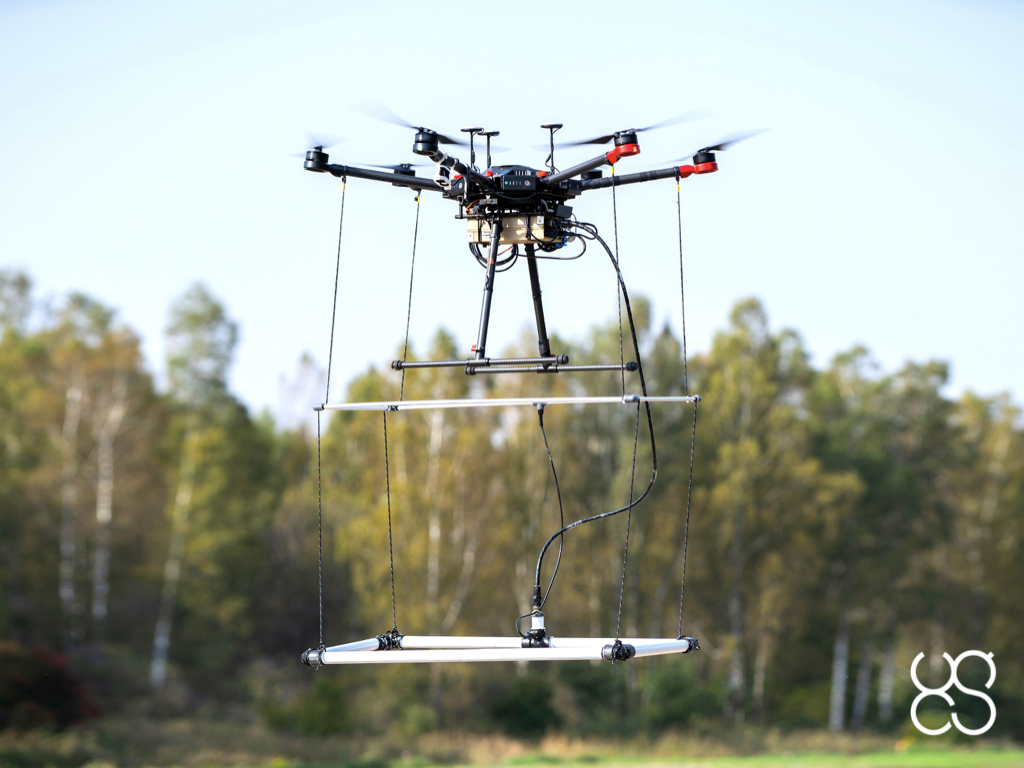
\includegraphics[width=\linewidth]{figs/Huirui/metal_detector_drone.png}
        \caption{UAV-mounted metal detector system\protect\footnotemark.}
        \label{fig:metal_detector_drone}
    \end{subfigure}
    \hfill
    \begin{subfigure}[b]{0.48\linewidth}
        \centering
        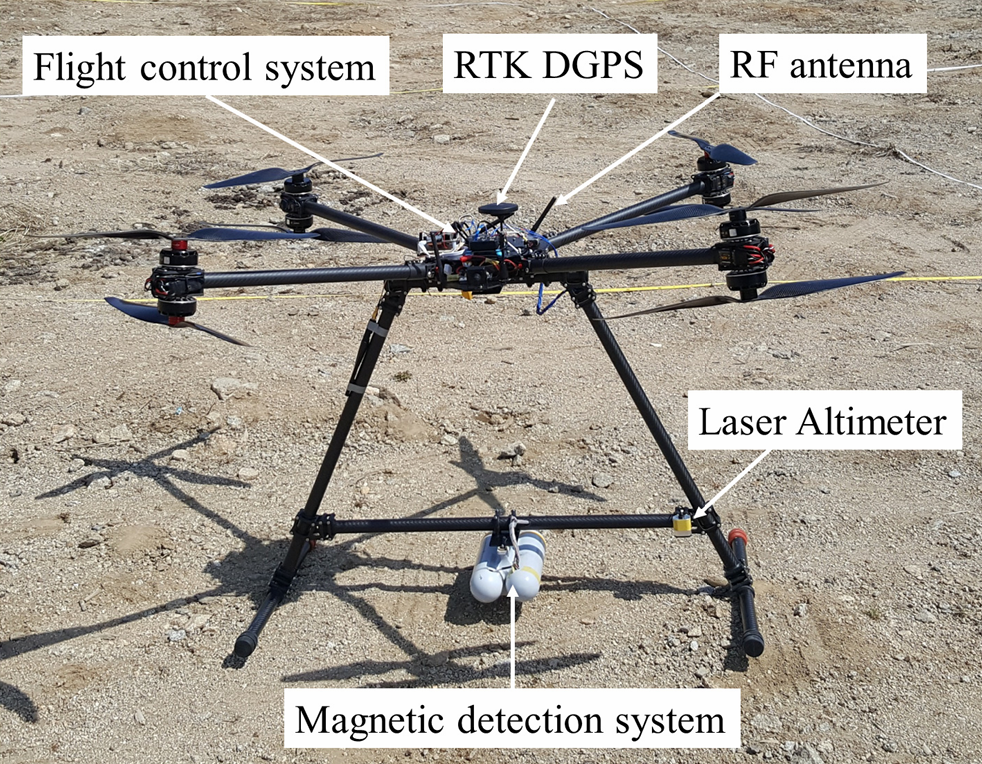
\includegraphics[width=\linewidth]{figs/Huirui/magnetometer_drone.png}
        \caption{Drone-based magnetometer platform~\cite{yoo2020drone}.}
        \label{fig:magnetometer_drone}
    \end{subfigure}
    \caption{Examples of UAV platforms integrating electromagnetic sensors for landmine detection.}
    \label{fig:emi_uav_examples}
\end{figure}

\footnotetext{\url{https://www.sphengineering.com/news/sph-engineering-introduces-the-drone-integrated-metal-detection-system}}

\paragraph{Radiowave and Microwave-Based Systems}

Ground Penetrating Radar (GPR) is a non-invasive geophysical technique that uses electromagnetic waves in the microwave frequency range (typically from several hundred MHz to a few GHz) to detect subsurface anomalies~\cite{gichd2006guidebook}. Unlike EMI-based systems, which respond to conductive or magnetic properties, GPR is sensitive to variations in the dielectric properties of materials~\cite{Gooneratne2004ARO}. It operates by transmitting short-duration radio pulses into the ground via a wideband antenna. When these pulses encounter boundaries between materials with different dielectric constants—such as between soil and a buried landmine—they are partially reflected. The reflected signals are then captured by a receiving antenna, and the time delay and intensity are analyzed to estimate the depth, shape, and dielectric contrast of subsurface targets~\cite{alqudsi2021review, paik2002image}.

As the antenna is moved across the ground, successive measurements are combined to construct two-dimensional slices (radargrams) or even three-dimensional volumetric representations of the subsurface~\cite{Bruschini1997ASO}. The effectiveness of GPR depends heavily on the contrast between the dielectric properties of the object and the surrounding soil. High-frequency systems offer better resolution and are more suited for detecting small anti-personnel mines, while lower-frequency systems provide deeper penetration but at the cost of detail~\cite{gichd2006guidebook}.

\textbf{Strengths:} One of GPR’s major strengths is its ability to detect both metallic and non-metallic mines, including those with plastic casings, by sensing changes in dielectric properties~\cite{Gooneratne2004ARO}. Unlike metal detectors, GPR systems are relatively insensitive to small surface metallic debris, which helps reduce false alarm rates~\cite{gichd2006guidebook}. They also provide useful information about object depth and shape, and can generate cross-sectional or 3D images of the subsurface~\cite{Bruschini1997ASO}. GPR is widely used in archaeological surveys, utility mapping, and geology, and is well understood in terms of commercial deployment and signal processing. Modern GPR systems are compact, lightweight, and pose no radiation hazard due to their low-power operation~\cite{gichd2006guidebook}.

\textbf{Limitations:} The main limitations of GPR lie in its sensitivity to soil conditions. High soil moisture, clay content, or rough surface topology can cause strong attenuation of the radar signal, making it difficult to detect shallow or low-contrast targets~\cite{Gooneratne2004ARO}. Performance can also degrade in dry, homogeneous soils due to insufficient dielectric contrast~\cite{robledo2009survey}. The detection of small anti-personnel mines can be particularly challenging if their signal is masked by surface reflections. Additionally, GPR systems require careful tuning of frequency to balance resolution and penetration depth, and are susceptible to signal distortion caused by subsurface clutter such as rocks, roots, or air pockets~\cite{cardonalandmine}.

\textbf{Drone-Based Applications:} GPR has been widely explored for drone integration due to its capability to detect plastic-cased mines and to provide volumetric subsurface data. UAV-mounted GPR systems typically use lightweight ultra-wideband (UWB) antennas and operate at low altitude to maintain signal fidelity. Applications include detecting anti-tank and anti-personnel mines in varied terrain types, including sand, loam, and clay\footnote{\url{https://www.sphengineering.com/integrated-systems/technologies/gpr}}~\cite{vsipovs2020lightweight,cerquera2017uav,fernandez2018synthetic,amiri2012feasibility,safarov2022detection,vsipovs2020lightweight,colorado2017integrated,schreiber2019advanced,pongrac2022advanced,garcia2020airborne,prager2019application,garcia2019autonomous,burr2018design,fernandez2021development,colorado2017low,lee2023modeling,sipos2017drone,garcia2022safedrone,almutiry2020uav,schartel2018uav,bahnemann2022under,garcia2022validation,chen2023ground}. Figure~\ref{fig:gpr_uav_examples} shows two UAV-based implementations of GPR for landmine detection.

\begin{figure}[h!]
    \centering
    \begin{subfigure}[b]{0.48\linewidth}
        \centering
        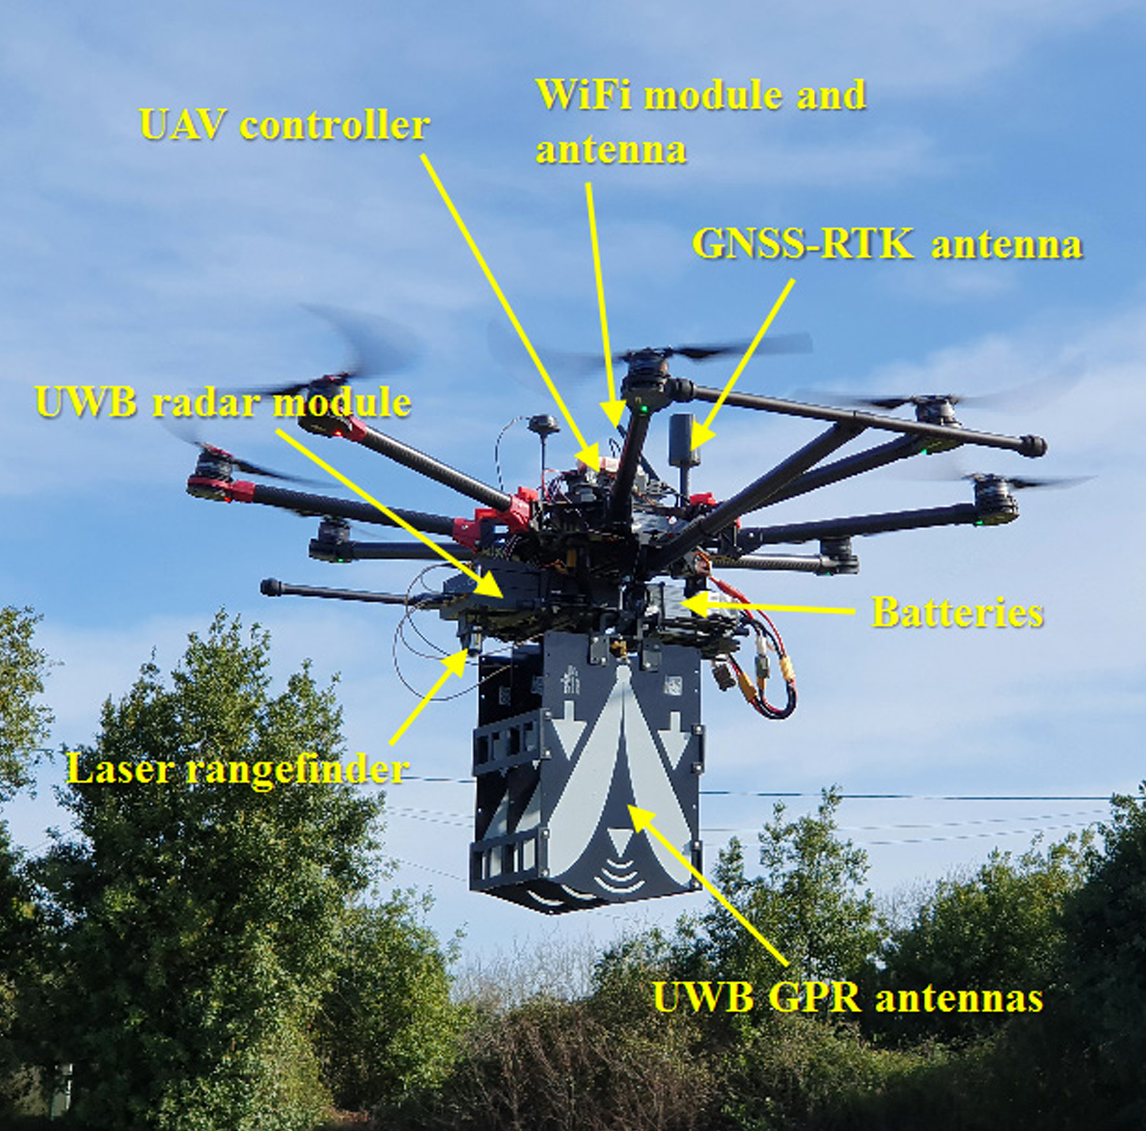
\includegraphics[width=\linewidth]{figs/Huirui/gpr_drone1.png}
        \label{fig:gpr_drone1}
    \end{subfigure}
    \hfill
    \begin{subfigure}[b]{0.48\linewidth}
        \centering
        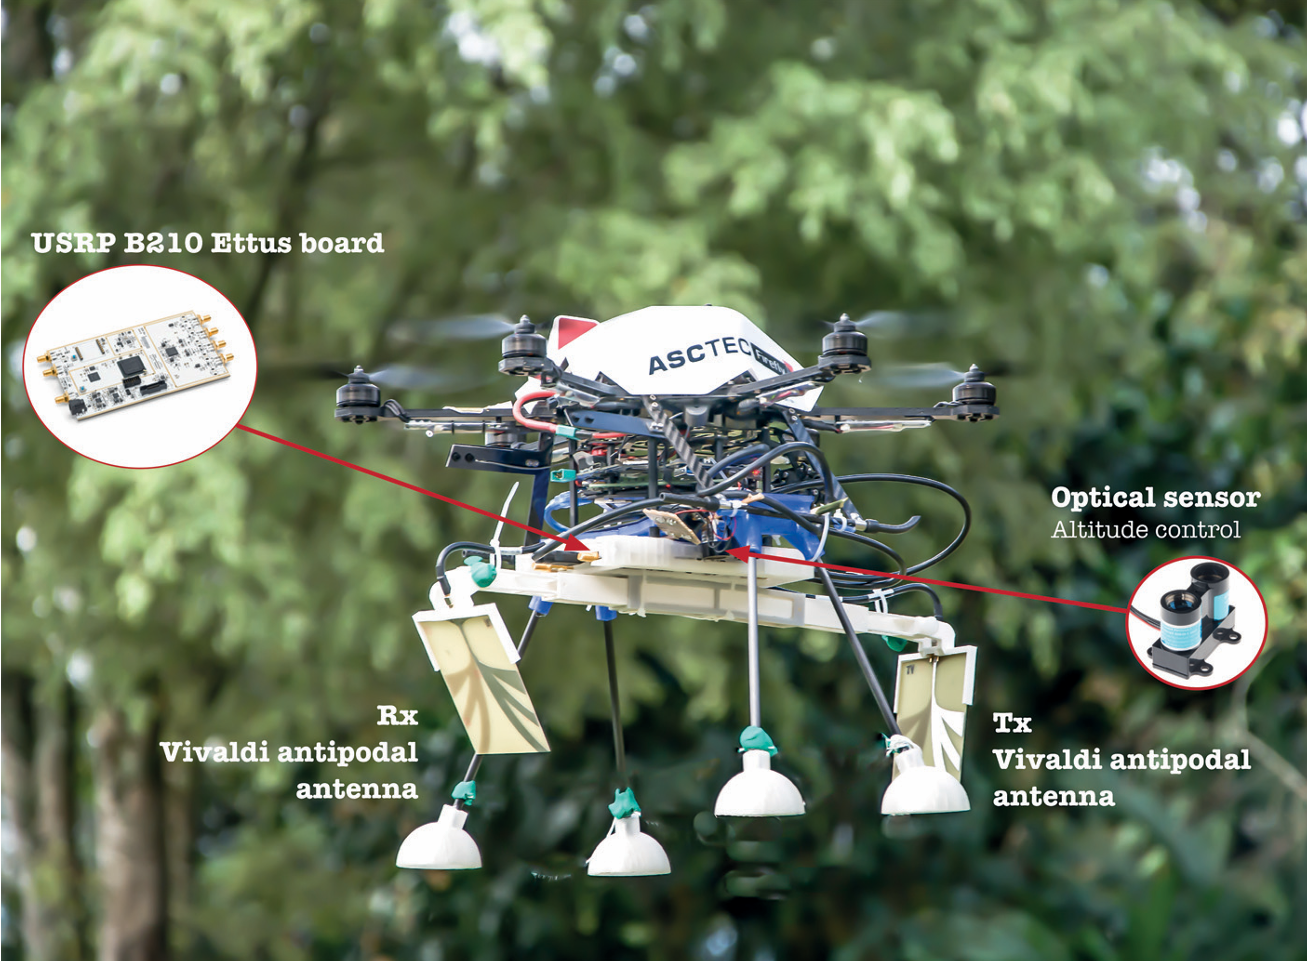
\includegraphics[width=\linewidth]{figs/Huirui/gpr_drone2.png}
        \label{fig:gpr_drone2}
    \end{subfigure}
    \caption{Examples of UAV platforms integrating GPR systems for landmine detection.~\cite{garcia2022safedrone,cerquera2017uav}}
    \label{fig:gpr_uav_examples}
\end{figure}

\paragraph{Spectral and Thermal Imaging Approaches}

Spectral and thermal imaging techniques detect anomalies in the electromagnetic radiation reflected or emitted from the Earth's surface. These methods aim to identify visual or thermal patterns associated with landmines or disturbed soil above them. The three primary sensor modalities in this class include visible-spectrum (optical) imaging, thermal infrared (IR) imaging, and hyperspectral or multispectral imaging.

\textbf{Optical cameras} operate in the visible light range and capture color or grayscale images of the terrain. They are primarily used to identify surface-laid landmines or areas with disturbed soil resulting from recent burial. These systems rely on texture and shape contrast, and their effectiveness depends on unobstructed ground visibility and minimal vegetation~\cite{cardonalandmine}.

\textbf{Thermal infrared imaging} detects differences in heat emissions between landmines and surrounding soil. Due to variations in thermal conductivity and heat capacity, mines retain or release heat at different rates, producing temperature contrasts that can be sensed with thermal cameras. These contrasts may arise from volume effects (influences on subsurface heat flow) or surface effects (soil disturbance from burial). Thermal infrared imaging is most effective during diurnal transitions, such as early morning or late evening~\cite{Bruschini1997ASO,paik2002image,hutsul2024review}.

\textbf{Hyperspectral and multispectral imaging} collect data across many discrete spectral bands, spanning the visible, near-infrared, and shortwave infrared regions. These sensors are used to detect subtle changes in soil composition, vegetation stress, or camouflage indicative of buried mines~\cite{robledo2009survey,alqudsi2021review}.

\textbf{Strengths:} All three imaging modalities are non-contact, passive, and lightweight, making them suitable for drone integration. They can scan large areas rapidly and are effective for detecting surface-laid or shallowly buried landmines under appropriate conditions. Optical imaging is particularly advantageous due to its low cost and simplicity. Thermal imaging excels in identifying subsurface anomalies caused by heat transfer, enabling detection of mines with limited surface visibility. Hyperspectral and multispectral systems provide detailed material and spectral information, enabling detection of subtle disturbances in the terrain or vegetation. These sensors are often used in conjunction with machine learning models to enhance detection accuracy.

\textbf{Limitations:} These technologies are all sensitive to environmental conditions such as lighting, cloud cover, surface moisture, and vegetation. Optical cameras cannot detect mines buried beneath the surface and are limited in cluttered or shaded environments~\cite{cardonalandmine}. Thermal cameras require favorable thermal gradients, and their effectiveness diminishes for deeply buried mines or under conditions that suppress temperature differences~\cite{Kovcs2022LandmineDW}. Hyperspectral and multispectral cameras, while informative, are unable to capture thermal emissions due to their shorter wavelength range.

\textbf{Drone-Based Applications:} UAV-based deployment of optical, thermal, and hyperspectral sensors has been demonstrated extensively for minefield surveying and detection~\cite{dena2020image,7529819,Schutte2001ARCAC,10.1117/12.2177182,Popov2022MethodFM,Desmet2018DronesA,rs15040967,10.1117/12.720442,Baur2021HowTI,baur2020applying,Stankevich2024OpticalAM,AgrawalChung2024ComparingSL,bajic2017developing,10765909,6842242,rs16040677,rs16122046,qiu2023joint,guo2022uav,ptsa-qj43-23,TENORIOTAMAYO2023109443,nikulin2018detection,FORERORAMIREZ2022104307,TENORIOTAMAYO2024105567,krause2018diurnal,Fardoulis2020PROOFHS,butt2024uav}.

\begin{figure}[h!]
    \centering
    \begin{subfigure}[b]{0.48\linewidth}
        \centering
        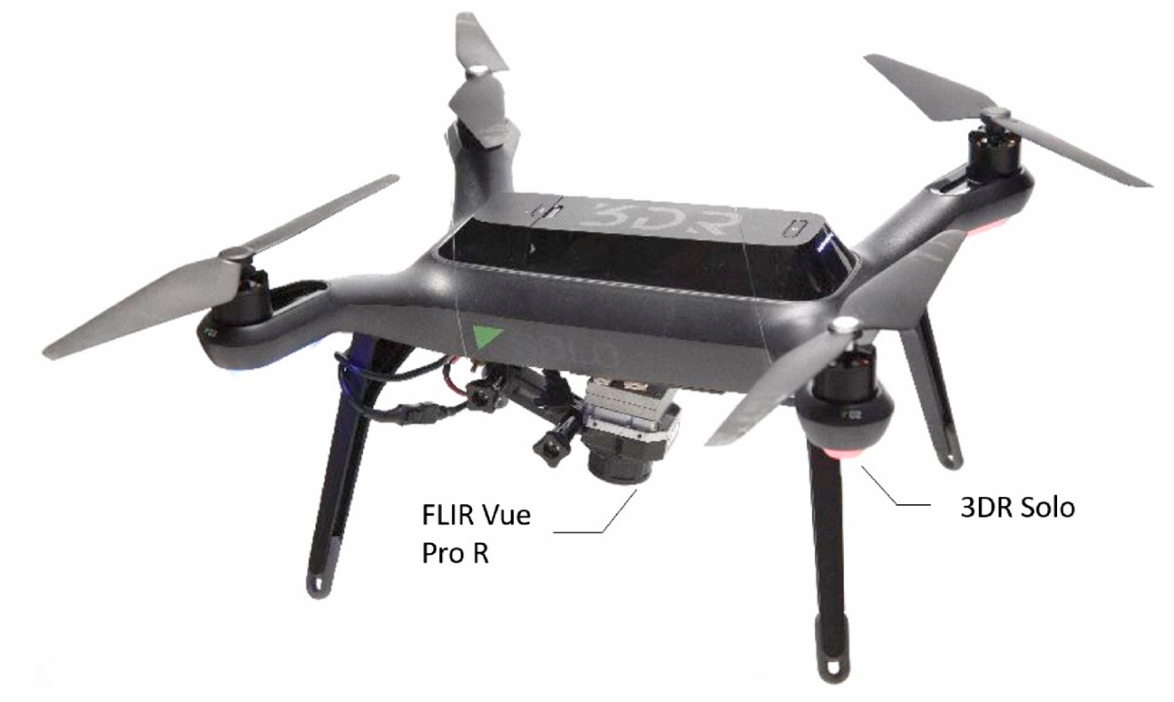
\includegraphics[width=\linewidth]{figs/Huirui/thermal_camera_drone.png}
        \caption{Thermal infrared camera mounted on UAV~\cite{nikulin2018detection}.}
        \label{fig:thermal_camera_drone}
    \end{subfigure}
    \hfill
    \begin{subfigure}[b]{0.48\linewidth}
        \centering
        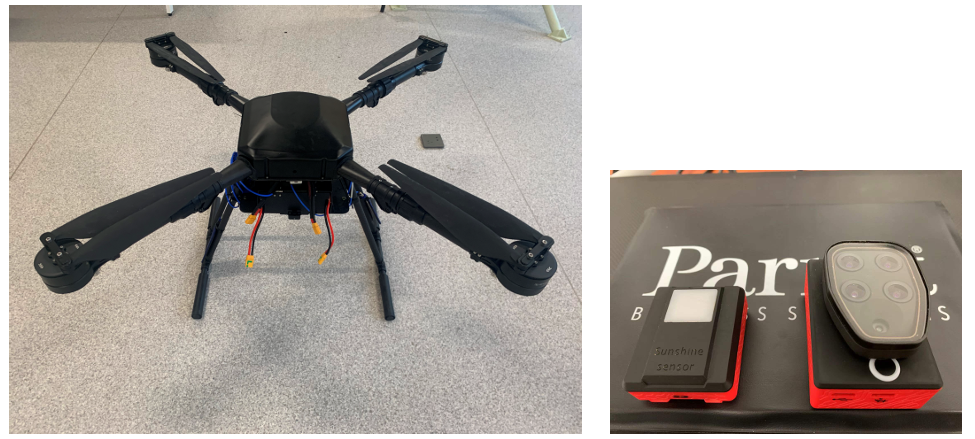
\includegraphics[width=\linewidth]{figs/Huirui/multispectral_drone.png}
        \caption{Multispectral camera mounted on UAV~\cite{qiu2023joint}.}
        \label{fig:optical_camera_drone}
    \end{subfigure}
    \caption{Examples of UAV-mounted spectral sensors used in landmine detection.}
    \label{fig:spectral_camera_drones}
\end{figure}


\paragraph{Mechanical and Vibro-Acoustic Methods}

This class includes detection technologies that exploit the mechanical or vibrational response of buried mines when stimulated by acoustic, seismic, or ultrasonic energy. These methods differ from electromagnetic and radar-based systems by relying on the physical compliance of buried objects rather than their electromagnetic properties~\cite{Gooneratne2004ARO,gichd2006guidebook}.

Acoustic and seismic techniques operate by transmitting low-frequency sound or seismic waves into the ground and measuring the reflected or re-radiated waves using contact or non-contact sensors. Mines are detected based on differences in their vibrational resonance, which contrasts with that of natural materials such as rocks, roots, or metal debris~\cite{gichd2006guidebook}. Similarly, ultrasound-based systems emit high-frequency acoustic waves (above 20 kHz) that reflect off material boundaries with different acoustic impedances. These reflections can be analyzed to image buried structures~\cite{paik2002image,cardonalandmine}.

\textbf{Strengths:} These methods are capable of detecting both metallic and non-metallic mines by exploiting their mechanical compliance~\cite{Gooneratne2004ARO}. They are largely unaffected by soil moisture, mineral content, or surface clutter, and offer a fundamentally different detection principle from electromagnetic methods. Acoustic systems have shown potential for reducing false alarm rates due to their ability to discriminate between man-made and natural subsurface materials~\cite{gichd2006guidebook}.

\textbf{Limitations:} Their effectiveness drops significantly for deeply buried targets or in hard, compacted, or frozen soils where wave propagation and resonance are suppressed. Laser Doppler vibrometers and other remote sensors may struggle in dense vegetation, and surface vibrations are often small and challenging to measure accurately. Ultrasound methods also suffer from strong attenuation at the air-soil interface, limiting their penetration depth and making them less suitable for non-contact UAV deployment~\cite{Gooneratne2004ARO,cardonalandmine}.

\textbf{Drone-Based Applications:} No practical implementations have been reported to date. Research in this area is still at an early conceptual stage, with ground-based systems dominating current development.

\paragraph{Chemical and Biological Sensing Methods}

These techniques target the detection of explosive compounds or their vapors emitted by buried landmines. The methods include chemical vapor sensors, biosensors, and systems utilizing trained animals or genetically engineered microorganisms~\cite{Gooneratne2004ARO,alqudsi2021review}.

Biological methods involve using animals such as dogs, rats, or bees, or genetically modified bacteria that fluoresce in the presence of explosive molecules like TNT. Bacteria-based systems can be sprayed over a suspected minefield and monitored later for fluorescence~\cite{cardonalandmine}. Chemical sensors, by contrast, use materials such as polymer arrays or photoluminescent compounds to detect vapor signatures of explosives~\cite{alqudsi2021review}.

\textbf{Strengths:} These methods can detect mines regardless of casing material, as they directly target the explosive itself~\cite{Gooneratne2004ARO,alqudsi2021review}. They are highly specific when tuned to particular compounds and can be developed into small, low-power devices for drone integration. Biological approaches like bacteria spraying offer wide-area coverage without the need for ground contact~\cite{cardonalandmine}.

\textbf{Limitations:} Environmental conditions such as humidity, temperature, and wind significantly affect vapor transport and detection reliability. Vapor concentrations are often extremely low and may be disturbed by UAV rotor downwash. Some biological methods (e.g., bacteria) are limited to TNT and cannot detect other common explosives like RDX or PETN~\cite{Gooneratne2004ARO,cardonalandmine}. Additionally, deployment logistics and false alarms from other soil contaminants remain concerns.

\textbf{Drone-Based Applications:} No fully developed or fielded systems have yet been reported in practice. Most developments in this area remain at the theoretical level.